\section{Anhang}

Im Anhang sind verschiedene Teile der Dokumentation gesammelt, die den Lesefluss im Hauptteil unnötig erschweren würden, und eher als Referenz denn zum Durchlesen gedacht sind.

Weiter sind hier im Anhang Dokumente aufgelistet, die mit der Arbeit im Zusammenhang stehen, aber nicht physisch mit diesem Dokument verbunden sein sollen.

\subsection{Systemspezifikation}

Bei \texttt{px} handelt es sich um ein modular aufgebautes Kommandozeilenprogramm. Der Code ist in zwei Teile eingeteilt: das \texttt{px}-Modul (Library), das die Funktionalität anwendungsneutral zur Verfügung stellt, und das Kommandozeilenprogramm \texttt{cmd/px.go}, das die kommandozeilenspezifischen Operationen (Interpretation der Parameter, Ein- und Ausgabe) übernimmt, und Gebrauch vom \texttt{px}-Modul macht.

\subsubsection{Systemkontext}
\label{sec:Systemkontext}

\begin{figure}
	\centering
	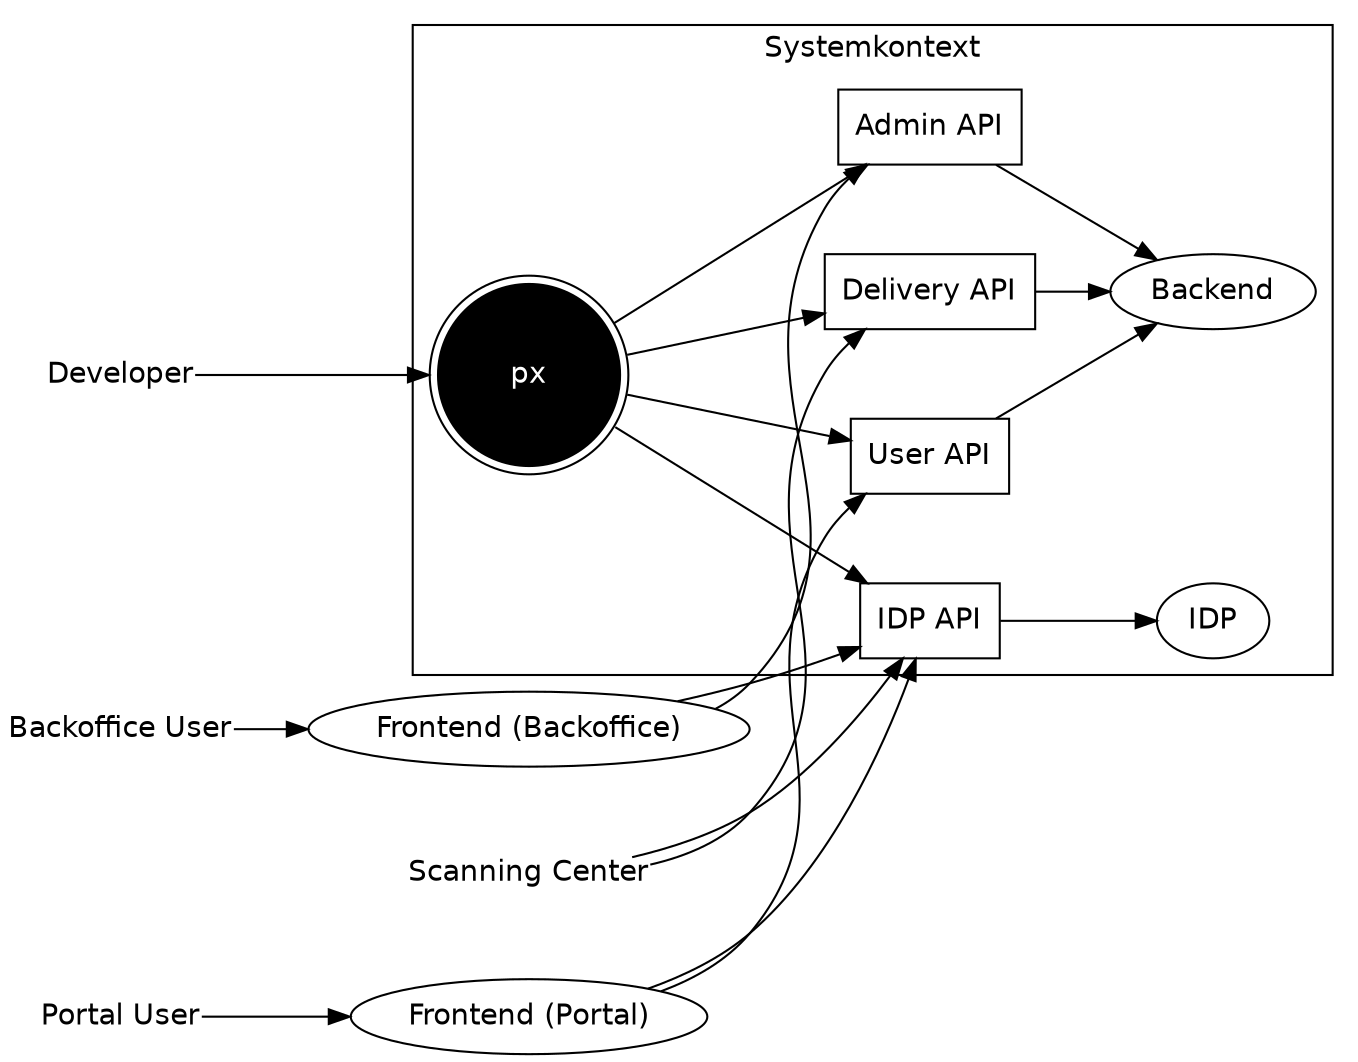
\includegraphics[width=\linewidth]{pics/kontextdiagramm.png}
	\caption{Kontextdiagramm: \texttt{px} als der Gegenstand der Arbeit innerhalb des Systemkontexts}
	\label{fig:kontextdiagramm}
\end{figure}

Im Kontextdiagramm (\imgref{fig:kontextdiagramm}) wird die zu entwickelnde Komponente \texttt{px} im Systemkontext von PEAX dargestellt. Andere Komponenten sind als Ellipsen, Schnittstellen als Rechtecke dargestellt. Ausserhalb vom Systemkontexts befindet sich die irrelevante Umgebung (d.h. die Frontend-Anwendungen). Die im Kontextdiagramm verwendeten Begriffe haben folgende Bedeutungen:

\begin{itemize}
	\item \texttt{px}: Der PEAX Command Line Client (Gegenstand der vorliegenden Arbeit)
	\item Developer: Ein Softwareentwickler (im weitesten Sinne) bei PEAX, der \texttt{px} verwendet.
	\item Backoffice User: Ein PEAX-Angestellter mit administrativen Befugnissen (Benutzerverwaltung).
	\item Portal User: Ein Benutzer des PEAX-Portals (Kunde).
	\item Scanning Center: Zulieferfirma, welche die umgeleitete Papierpost der PEAX-Kunden erhält, diese einscannt und dem betreffenden Kunden ins Portal stellt.
	\item Frontend (Backoffice): Ein Web-GUI für administrative Tätigkeiten zum internen Gebrauch.
	\item Frontend (Portal): Ein Web-GUI für die Kunden von PEAX (das eigentliche Portal).
	\item Admin API: RESTful API für administrative Aufgaben
	\item Agent API: RESTful API zum Einliefern von Dokumenten über Zulieferer
	\item User API: RESTful API für die Operationen der Kunden
	\item IDP API: RESTful API für das Token-Management (OAuth 2.0/OpenID Connect)
	\item Backend: Serverseitige Software mit Businesslogik und Datenspeicher
	\item IDP: Identity Provider, API-übergreifende Benutzer- und Zugangsverwaltung (AuthN/AuthZ)
\end{itemize}

\subsection{Technologie-Evaluation}

- Vorgabe: PEAX API (RESTful)

\subsubsection{Programmiersprache}

Aus der Aufgabenstellung und dem Umfeld bei PEAX ergeben sich folgende nicht-funktionale Anforderungen an die zu erstellende Software:

\begin{description}
    \item[Installation] Die Software soll sich einfach installieren lassen.
    \item[Umgebung] Es dürfen keine besonderen Anforderungen an die Umgebung gestellt werden, auf der \texttt{px} läuft.
    \item[Plattformen] Die Software soll auf allen gängigen, d.h. bei PEAX eingesetzten, Betriebssystemen (\textsc{Windows}, \textsc{macOS}, \textsc{Linux}) lauffähig sein.
    \item[Einheitlichkeit] Der Client soll überall die gleiche Befehlssyntax haben.
    \item[Performance] Ein Command Line Client soll in Skripten verwendet werden können, wodurch das Programm sehr oft in kurzem Zeitraum aufgestartet werden muss.
\end{description}

\textsc{Java}, das bei PEAX im Backend-Bereich zum Einsatz kommt, erfordert die lokale Installation einer JRE in der richtigen Version, was bei Frontend-Entwicklern nicht gegeben ist. Ausserdem werden Wrapper-Skripts benötigt (\texttt{java -jar px.jar} ist nicht praktikabel).

\textsc{Python}, \textsc{Ruby}, \textsc{Perl} und andere Skriptsprachen benötigen ebenfalls einen vorinstallierten Interpreter in der richtigen Version.

Zwar gibt es mit Mono eine Variante von .Net, die überall lauffähig ist, hier werden aber wiederum eine Laufzeitumgebung bzw. vorinstallierte Libraries benötigt.

Für die Problemstellung am besten geeignet sind kompilierte Sprachen (C, C++, \textsc{Go}, \textsc{Rust}, \textsc{Nim}). Mit einer statischen Kompilierung lässt sich das ganze Programm in eine einzige Binärdatei überführen, welches denkbar einfach zu installieren ist (Kopieren nach einem der Verzeichnisse innerhalb von \texttt{\$PATH}).

Für \textsc{JavaScript}, das bei PEAX im Frontend zum Einsatz kommt, gibt es mit \textsc{QuickJS}\footnote{\url{https://bellard.org/quickjs/}} seit kurzem die Möglichkeit, \textsc{JavaScript} zu Binärdateien zu kompilieren. Dies funktioniert aber nicht auf allen Plattformen, ausserdem ist \textsc{QuickJS} noch experminentell und noch nicht für den produktiven Einsatz geeignet.

Um ein Projekt vom gegebenen Umfang innerhalb eines Semesters umsetzen zu können, sind Vorkenntnisse in der einzusetzenden Programmiersprache zwar nicht zwingend, können das Risiko des Scheiterns aber erheblich senken. Gerade bei der Abschätzung von Aufwänden ist Vertrautheit mit den einzusetzenden Werkzeugen sehr hilfreich.

Was (statisch) kompilierte Programmiersprachen betrifft, konnte der Autor dieser Arbeit bereits Erfahrungen mit C, \textsc{Go} und \textsc{Rust} sammeln. Das manuelle Speichermanagement in C (u.a. auch bei Strings) ist einerseits ein grosses Risiko (Buffer Overflows, Segmentation Faults), und wirkt sich andererseits negativ auf das Entwicklungstempo aus. In die engere Auswahl kommen somit \textsc{Go} und \textsc{Rust}.

Im Folgenden werden die gemachten Erfahrungen und die dabei empfundenen Vor- und Nachteile mit den Programmiersprachen \textsc{Go} und \textsc{Rust} einander gegenübergestellt.

\subsubsection{\textsc{Go}}

Mit \textsc{Go} konnte der Autor dieser Arbeit bereits einges an Erfahrung sammeln. So wurde neben dem Prototyp zu \texttt{px} bereits die Testat-Aufgabe im Modul Software Testing\footnote{\url{https://github.com/patrickbucher/getting-to-philosophy}}, ein Thumbnailer\footnote{\url{https://github.com/patrickbucher/thumbnailer}} sowie zahlreiche Utilities\footnote{\url{https://github.com/patrickbucher/go-scratch}} (viele darunter als HTTP-Clients) in \textsc{Go} entwickelt. Dabei wurden folgende Vor- und Nachteile ermittelt:

\begin{itemize}
    \item[+] aufgrund weniger Keywords und Features einfach zu lernen
    \item[+] hervorragendes Tooling out-of-the-box
    \item[+] Cross-Compilation ohne Zusatztools auf alle unterstützte Plattformen möglich
    \item[+] schnelle Kompilierung
    \item[+] umfassende Standard-Library, die u.a. ein hervorrangendes HTTP-Package beinhaltet
    \item[+] persönlich bereits viel (positive) Erfahrungen damit gesammelt
    \item[+] wird bereits für andere bei PEAX gebräuchliche CLI-Tools eingesetzt (\texttt{oc}, \texttt{docker})
    \item[+] fügt sich sehr gut in die \textsc{Unix}-Philosophie ein (Tooling, Libraries)
    \item[+] Einfaches Interface für nebenläufige Programmierung (Goroutines und Channels)
    \item[+] geringer Memory-Verbrach bei relativ hoher Performance\footnote{\url{https://benchmarksgame-team.pages.debian.net/benchmarksgame/fastest/go.html}}
    \item[-] keine Features wie Generics, Exceptions und \texttt{filter}/\texttt{map}/\texttt{reduce}
    \item[-] Binaries fallen relativ gross aus\footnote{\url{https://golang.org/doc/faq\#Why\_is\_my\_trivial\_program\_such\_a\_large\_binary}}
    \item[-] Error-Handling aufwändig und teils repetitiv
\end{itemize}

\subsubsection{\textsc{Rust}}

Der Autor dieser Arbeit konnte sich bereits letztes Jahr im Rahmen des Moduls \textit{Programming Concepts and Paradigms} an der HSLU Informatik mit \textsc{Rust} befassen \cite[S. 12]{pcp-rust}. Nach selbständiger Beschäftigung mit dieser Programmiersprache im Sommer können (teils ergänzend) folgende Vor- und Nachteile genannt werden:

\begin{itemize}
    \item[+] viele moderne Features (Generics, \texttt{filter}/\texttt{map}/\texttt{reduce})
    \item[+] hervorragendes Typsystem
    \item[+] gutes und ausgereiftes Tooling
    \item[+] weder manuelles Memory-Management noch Garbage Collector nötig
    \item[+] Pattern Matching führt zu sehr solidem Code
    \item[+] gegenüber \textsc{Go} schlankere Binaries
    \item[+] kommt bereits in der Form einiger CLI-Tools persönlich zum Einsatz (\texttt{rg}, \texttt{bat}, \texttt{hexyl}, \texttt{battop})
    \item[+] erstklassige Performance (im Bereich von C/C++) bei geringem Speicherverbrauch\footnote{\url{https://benchmarksgame-team.pages.debian.net/benchmarksgame/fastest/rust-go.html}}
    \item[-] hohe Einstiegshürde und lange Einarbeitungszeit
    \item[-] Cross-Compilation benötigt Zusatztools
    \item[-] noch keine praxisnahe Erfahrung damit gesammelt
    \item[-] aufgrund schlanker Standard Library auf viele Dependencies angewiesen
\end{itemize}

\subsubsection{Entscheidung Programmiersprache}
\label{sec:Entscheidung-Programmiersprache}

\textsc{Rust} hat gegenüber \textsc{Go} einige unbestreitbare Vorzüge (Memory Management, Typsystem, Ausdrucksstärke, Eliminierung ganzer Fehlerklassen, Performance, schlankere Binärdateien). Bezogen auf das umzusetzende Projekt haben jedoch einige davon kaum einen wichtigen Stellenwert (etwa Performance und Zero-Cost Abstractions). Hier fallen die Vorzüge von \textsc{Go} (umfassende Standard Library, Cross-Compilation) wesentlich stärker ins Gewicht.

Gerade die absichtlich schlank gehaltene Standard Library von \textsc{Rust}, die etwa zur Generierung von Zufallszahlen bereits externe Abhängigkeiten erfordert\footnote{\url{https://doc.rust-lang.org/book/ch02-00-guessing-game-tutorial.html\#using-a-crate-to-get-more-functionality}}, dürfte sich im vorliegenden Projektrahmen negativ auswirken, zumal die Evaluation verschiedener Libraries einen sehr hohen Zusatzaufwand erfordert.

Da \textsc{Go} bereits bei der Entwicklung des Prototypen von \texttt{px} erfolgreich zum Einsatz kam, und einige Projektaspekte (grundlegende CI-Pipeline, \texttt{Makefile} für Cross-Compilation und Packaging) bereits damit implementiert werden konnten, soll \textsc{Go} für das vorliegende Projekt den Vorzug erhalten.

Eine spätere Neuimplementierung von \texttt{px} in \textsc{Rust} wäre ein technisch durchaus interessantes, wenn auch praktisch wenig dringendes ‒ als Fallstudie aber durchaus lohnendes ‒ Unterfangen.

\subsection{Libraries}

TODO: JWT, Keystore, Password Input

\subsection{Weitere Dokumente}
\label{apx:WeitereDokumente}

\begin{description}
    \item[Projektauftrag] Im Projektauftrag (\texttt{Anhang/Projektauftrag.pdf}) ist die Aufgabe beschrieben, wie sie zu Beginn des Projekts definiert worden ist.
    \item[Projektplan] Der Projektplan (\texttt{Anhang/Projektplan.pdf}) besteht aus einem Rahmenplan, einem Meilensteinplan und einem Wochenplan.
    \item[Backlog] Das Backlog (\texttt{Anhang/Backlog.pdf}) enthält die einzelnen User Stories, die Sprint-Planung, Umsetzungsnotizen zu einzelnen User Stories und Testprotokolle dazu. 
    \item[Meilensteinbericht 1] Der erste Meilensteinbericht (\texttt{Anhang/Meilensteinbericht-1.pdf}) beschreibt die Vorgeschichte des Projekts und die Phase der Projektinitialisierung.
    \item[Meilensteinbericht 2] Der zweite Meilensteinbericht (\texttt{Anhang/Meilensteinbericht-2.pdf}) umfasst die ersten beiden Sprints.
    \item[Meilensteinbericht 3] \texttt{Anhang/Meilensteinbericht-3.pdf}
    \item[Arbeitsjournal] Im Arbeitsjournal (\texttt{Anhang/Arbeitsjournal.pdf}) sind die einzelnen Aufwände auf halbe Stunden gerundet nach Bereich ‒ Projekt(administration), Dokumentation, Umsetzung ‒ rapportiert. Mithilfe eines AWK-Skripts können die Aufwände nach Bereich und User Story ausgewertet werden.
\end{description}
